%!TEX root = ../../main.tex
%----------------------------------------------------------------------------
\chapter{System Test}\label{chap:system_test_chapter}
%----------------------------------------------------------------------------

% Please keep sections separated in their designated folders and only reference them here using the input tag

In order to prove the capabilities of out design and to bring all the so far undetected bugs and errors to light, we were asked to perform a 24-hour integration test. During this 24 hours, all components of the system had to be used throughout multiple iteration of the brick selection and delivery procedure. 

Since the timespan of the test was such that it encapsulated a whole day, the systems had to cope with changing light conditions, continuous interference by human operators and spectators moving around them, the degradation of markers essential for navigation while being forced to interact with other system components, the mobile platforms of the other groups. In the following sections we present a detailed description of the tests we performed, the results we got and their evaluation.


\section{Test description}

In the beginning of the test, all mobile platforms were situated at the charging stations, fully charged. One iteration consisted ot the following milestones:

\begin{enumerate}
	\item Leaving the charging station in a fully charged state and taking up position under the LEGO dispenser machine
	\item Waiting for the bricks to be loaded on the tipper (since the dispenser was not operational, we just simulated the process)
	\item Delivering the LEGO to the robot cell
	\item Unloading the bricks to the conveyor belt
	\item Moving the bricks into position for selection through robotic vision
	\item Picking the LEGO bricks specified by the order (this is equivalent to loading them on the mobile platform)
	\item Trafficking the LEGO back to the box, and docking at the charger
\end{enumerate}

All components of the system were continuously broadcasting location and status information, which was displayed on the HMI, while the map used for SLAM navigation and the console-printed ROS information were also monitored. We compared all these with the actual position and behavior of the system components, logged their performance, and intervened when errors occurred. 

\section{Log}

We logged the date and time, the person  responsible for creating the entry, the type of the entry and a short note describing the reason for making it.

We have distinguished between the following types:

\begin{itemize}
	\item Order Start
	\item Order Finish
	\item Error
	\item Manual Shutdown
	\item System Event
	\item Other
\end{itemize}


\section{Test results}

Even though in the initial phase camera connection issues caused delays in the testing process, all in all 49 iterations were performed, out of which 36 were finished successfully resulting in a success ratio of 73.47\% (see Figure \ref{fig:order_statistics} ).

\begin{figure}[H]
    \centering
    \begin{subfigure}[b]{0.48\textwidth}
        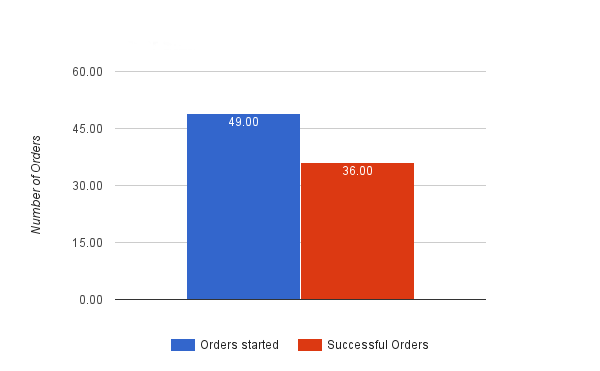
\includegraphics[width=\textwidth]{order_statistics}
        \caption{Order statistics}
        \label{fig:order_statistics}
    \end{subfigure}
    ~
    \begin{subfigure}[b]{0.48\textwidth}
        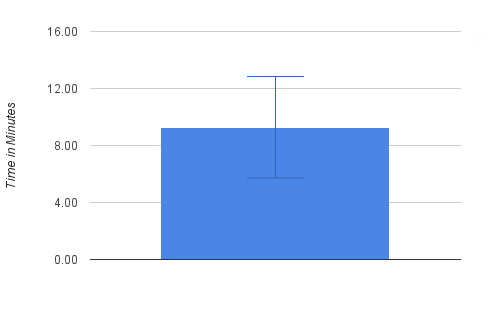
\includegraphics[width=\textwidth]{execution_time}
        \caption{Execution time}
        \label{fig:execution_time}
	\end{subfigure}
\caption{Test statistics}
\end{figure}

We managed to improve the speed of the system throughout the testing and on average we achieved an execution time of  9.28 minutes with a standard deviation of 3.35 (see Figure \ref{fig:execution_time}).

The two main sources of errors we have observed were originated in inter-component communication and the localization of the mobile platform. Since both are effected greatly by external factors such as congestion and uncontrollable changes in the environment caused by human and mobile robot movement, they cannot be mitigated without introducing fundamental changes to the design. 

Nevertheless, the fact, that after the initial difficulties no mayor errors occurred shows, that the corrected system is mostly bug free and a capable solution for the task presented.





%%% Local Variables:
%%% mode: latex
%%% TeX-master: "main"
%%% End: